\scanpage{68}\mspage{67}
\deleted{We have a notion of \unsure{``c|``C|``6}}

Every subset of $\mathcal F$ (resp $M$) is contained in a \unsure{minimal} saturated subset (among \unsure{such|those} containing it) which \deleted{is called \unsure{of the|of}} is none other than the cosupport of the cosupport, and is also called its support. The saturated subsets are those which are equal to the support, or to the cosupport, of a subset. The map . $\operatorname{cosup}$ \unsure{defines|defines} a \unsure{bij\inserted{e}ction} of the set of \unsure{saturated|saturated} subsets onto themselves, reversing the inclusion relation.

We denote by $\Sigma$ the set of \uline{virtual} \uline{supports}, or saturated subsets
% Figure R1-F1: raised M_0 and its curved oblique insertion leader, without arrowhead.
\figure{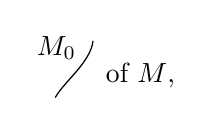
\begin{tikzpicture}[x=1cm,y=1cm]
  \node[anchor=base west] at (0,0) {of $M$,};
  \node[anchor=base east] at (-0.13,0.34) {$\inserted{M_0}$};
  \draw[line width=0.45pt] (-0.52,-0.19) .. controls (-0.40,0.02) and (-0.07,0.26) .. (-0.04,0.53);
\end{tikzpicture}}
where \deleted{\unsure{of}} $\mathcal F_0$ of $M$. \deleted{We \unsure{define}} \deleted{The cosupport map \unsure{d|of}} We \unsure{disidentify} $\Sigma$ from \deleted{$\unsure{\mathscr P|\mathcal F_2|\mathcal F_0|\mathcal F}$} its two 
% Two detached points beneath the word, with no inferred function.
\figure{%
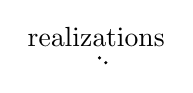
\begin{tikzpicture}[x=1cm,y=1cm]
\node[anchor=base west,inner sep=0] at (0,0) {\unsure{realizations}};
\fill (0.92,-0.14) circle[radius=0.022cm];
\fill (1.00,-0.20) circle[radius=0.022cm];
\end{tikzpicture}%
}
 (as \unsure{subset|subsets} of $\unsure{P|\mathscr P|\mathcal P}(M)$, or of $\mathscr P(\unsure{\mathcal F|F})$) and we write, for $\sigma\in\Sigma$
\[
M_\sigma\subset M,\qquad\mathcal F_\sigma\subset\unsure{\mathcal F|F}
\]

In $\Sigma$, \deleted{for} the notion of cosupport is an anti\unsure{\deleted{invo}lution|involution|bijection|duality} of ordered sets. In $\Sigma$, we have arbitrary $\mathrm{Inf}$ (it is the intersection of the subsets of $M$, or of $\mathcal F$), and arbitrary $\mathrm{Sup}$ (it is the saturated subset
